\documentclass{article}
\usepackage[utf8]{inputenc}
\usepackage[russian]{babel}
\usepackage{amsmath}
\usepackage{graphicx, color}

\begin{document}

\begin{titlepage}

\thispagestyle{empty}

\centerline{\Large{Федеральное государственное бюджетное}}
\centerline{\Large{образовательное учреждение высшего образования}}
\centerline{\Large{Московский государственный университет}}
\centerline{\Large{имени М.В.Ломоносова}}

\vfill

\centerline{\huge{Задача на простейшую работу с изображениями}}

\vfill
\vfill

Работу выполнила \hfill Комолова М.М.

Преподаватель \hfill Почеревин Р.В.

\vfill

\centerline{Москва, 2022}
\clearpage
\end{titlepage} 

\newpage
\section{Постановка задачи}
 
Программа должна загрузить изображение из графического файла
{\em InputFile\/}, изменить яркость изображения в {\em K1\/} раз и контраст в {\em K2\/} раз
и вывести получившееся изображение в графический файл {\em OutputFile\/}.
Под яркостью пиксела подразумевается сумма компонент пиксела.
\\
\section{Алгоритм}

{\bf Изменение яркости\/}
\\Яркость --- сумма компонент пикселя. Для изменения яркости в K1 раз нужно умножить каждую из компонент RGB на данный коэффициент K1. Формула:
$$b_{i}^{'} = b_{i}\cdot K1$$ где $b_{i}^{'}$ --- новое значение пиксела, а $b_{i}$ --- старое.
\\
\\
{\bf Изменение контраста\/}
\\Контраст --- отношение самого темного к самому яркому пикселю. При его увеличении темные участки становятся темнее, а светлые светлее. Для изменения контраста в K2 раз используем формулу:
$$b_{i}^{'} = (b_{i}-m_{i})\cdot K2+m_{i}$$ $$m_{i} = \frac {\sum\limits_{i = 0}^{h\cdot w}b_{i}}{h\cdot w}$$ где $h$ и $w$ --- количество пикселей в высоту и ширину картинки соответственно.

\newpage
\section{Примеры}

{\bf До изменения\/} \\
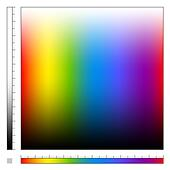
\includegraphics[totalheight = 4cm]{1.png} \hspace{1.5cm}
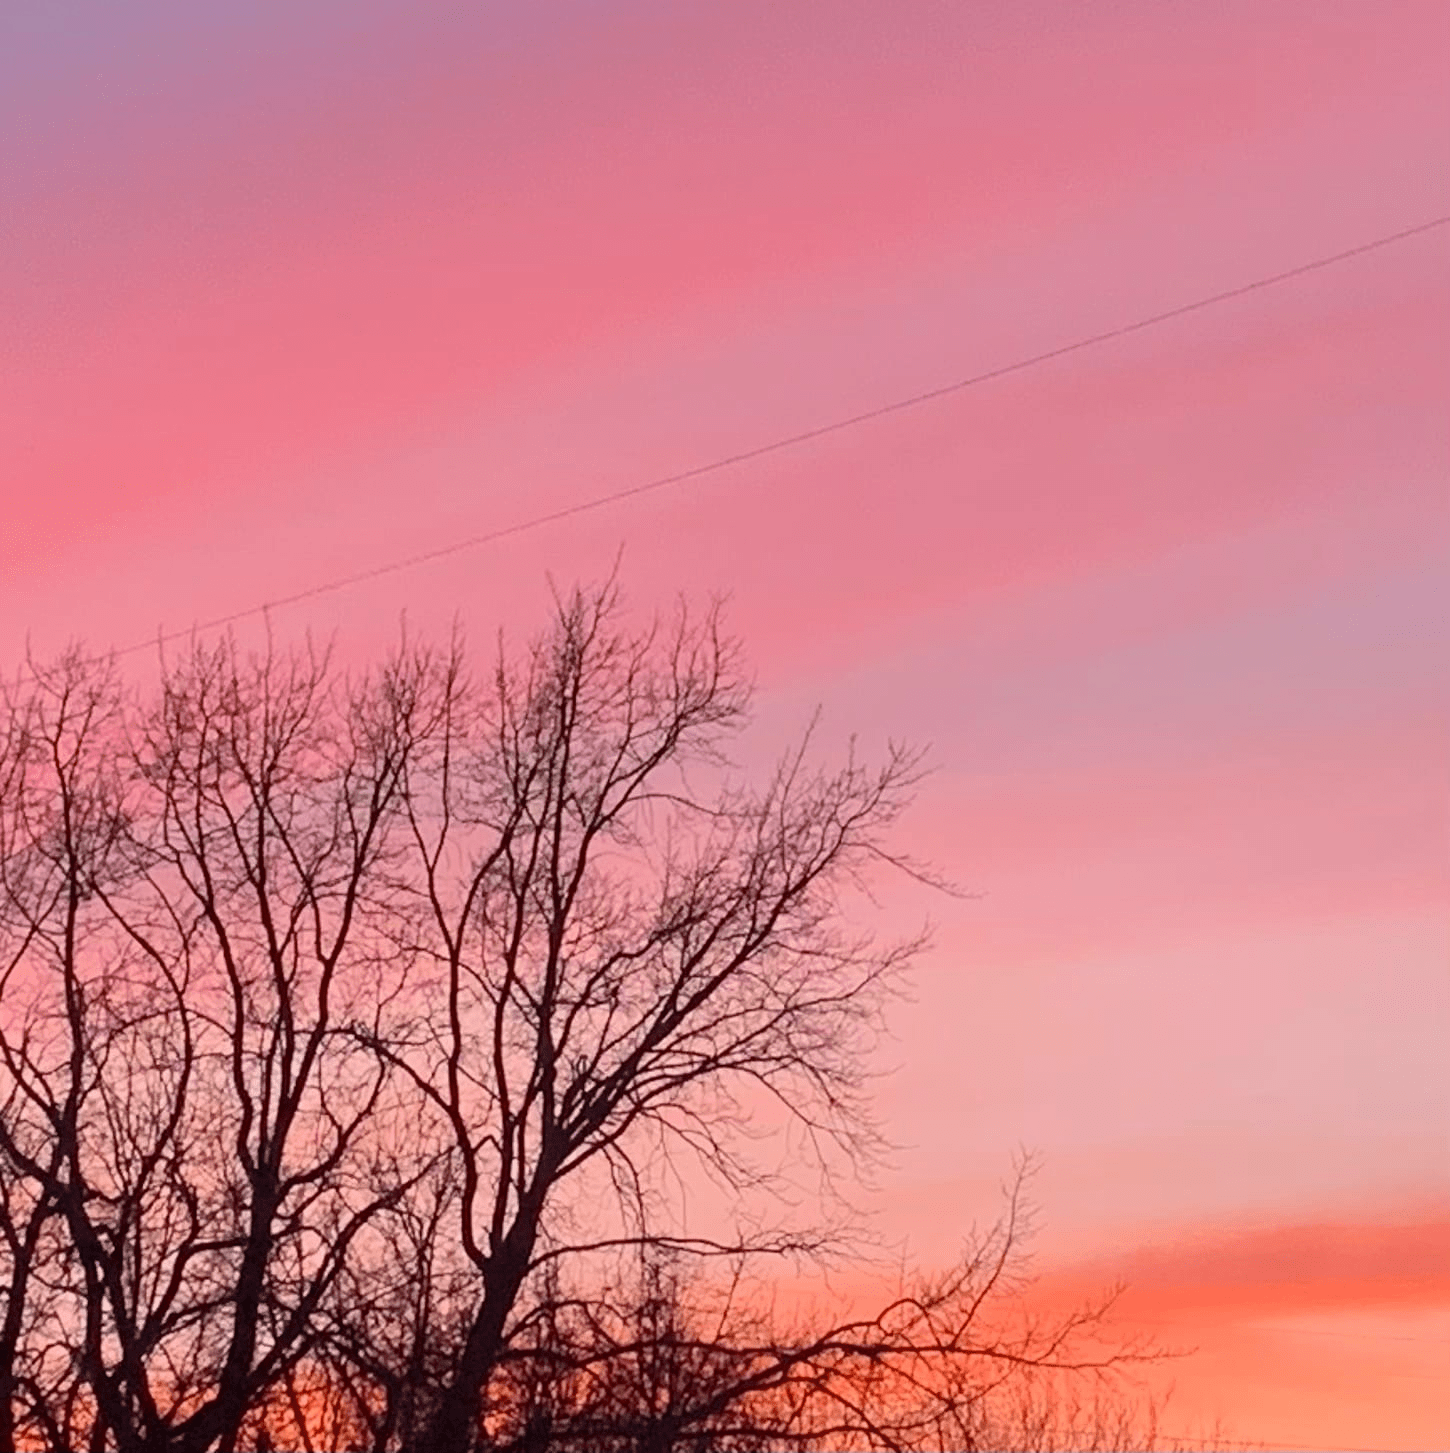
\includegraphics[totalheight = 4cm]{2.png} \hspace{1.5cm}

\includegraphics[totalheight = 4cm]{3.png} \\
{\bf K1 = 1, K2 = 2\/}\\
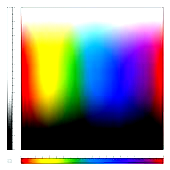
\includegraphics[totalheight = 4cm]{112.png} \hspace{1.5cm}
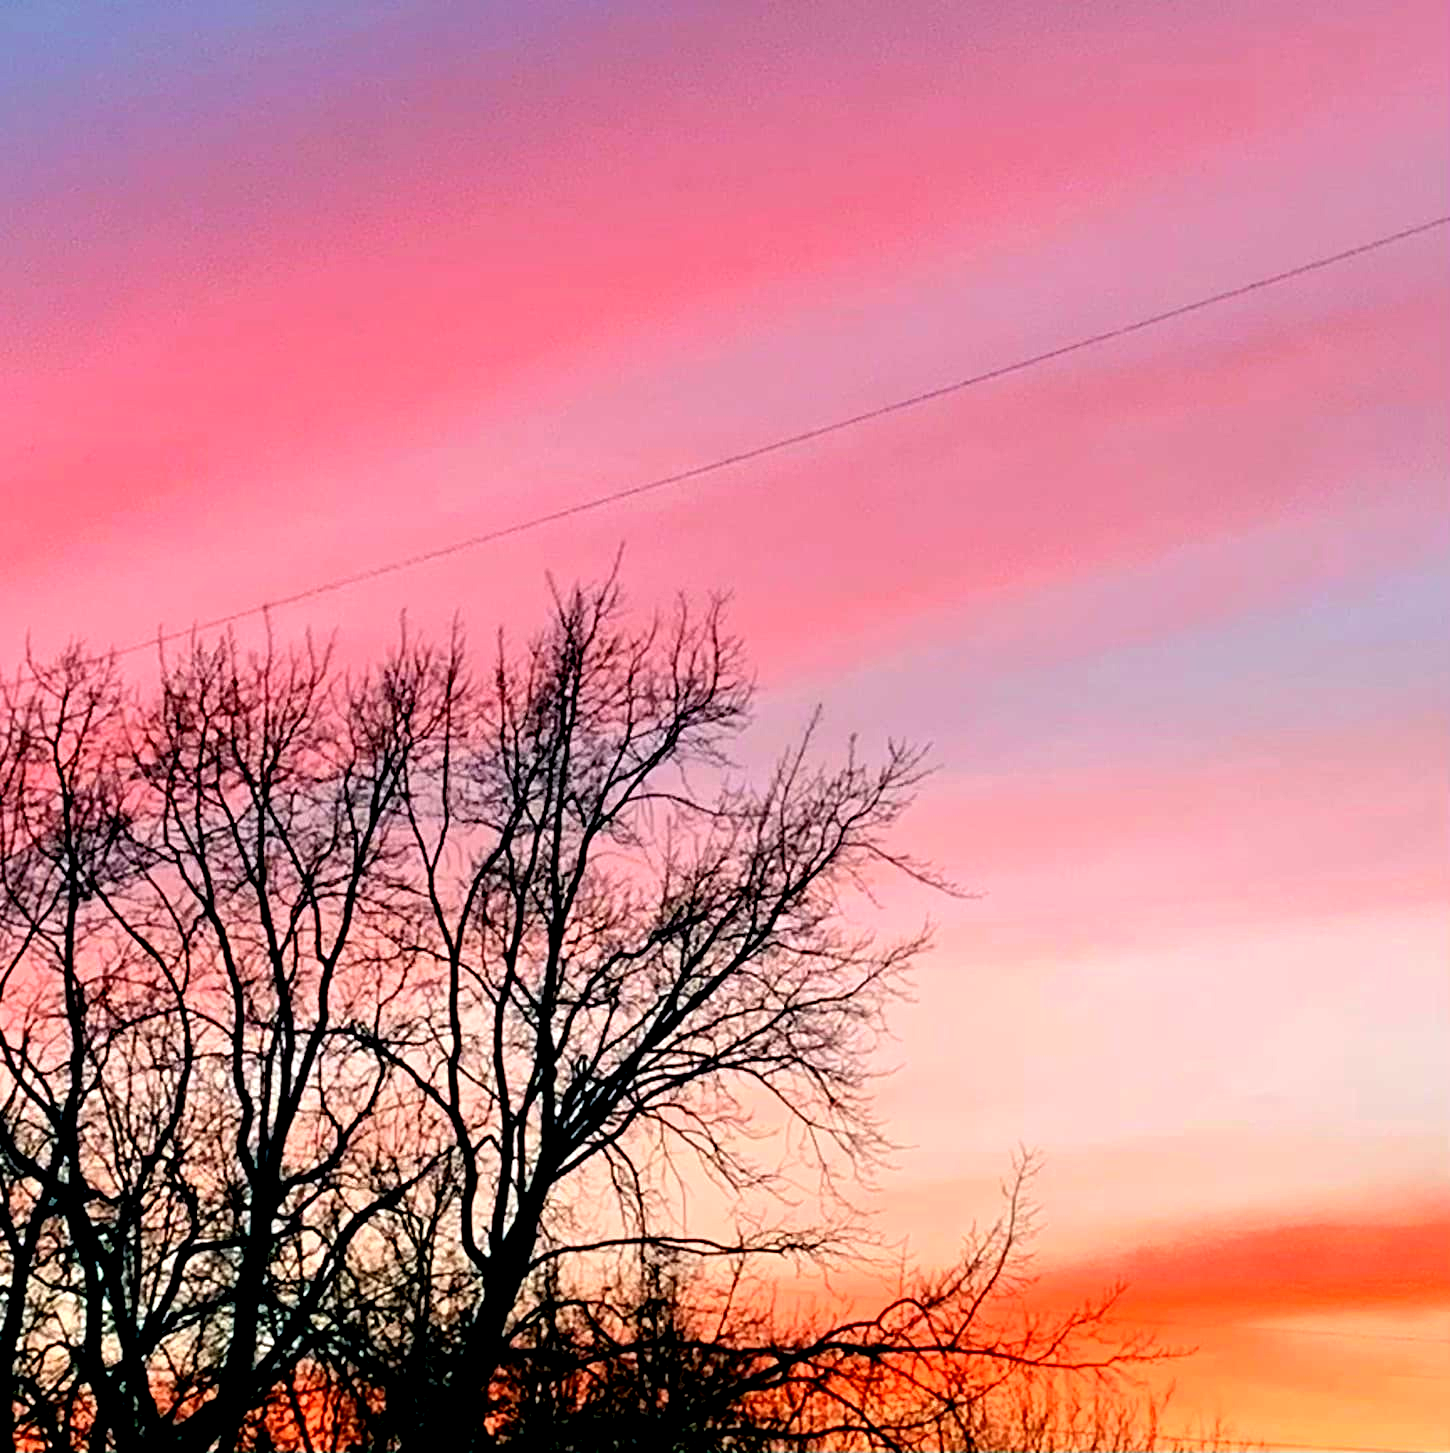
\includegraphics[totalheight = 4cm]{212.png} \hspace{1.5cm}

\includegraphics[totalheight = 4cm]{312.png} \\
{\bf K1 = 2, K2 = 1\/}\\
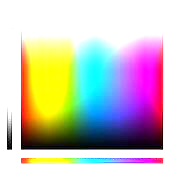
\includegraphics[totalheight = 4cm]{121.png} \hspace{1.5cm}
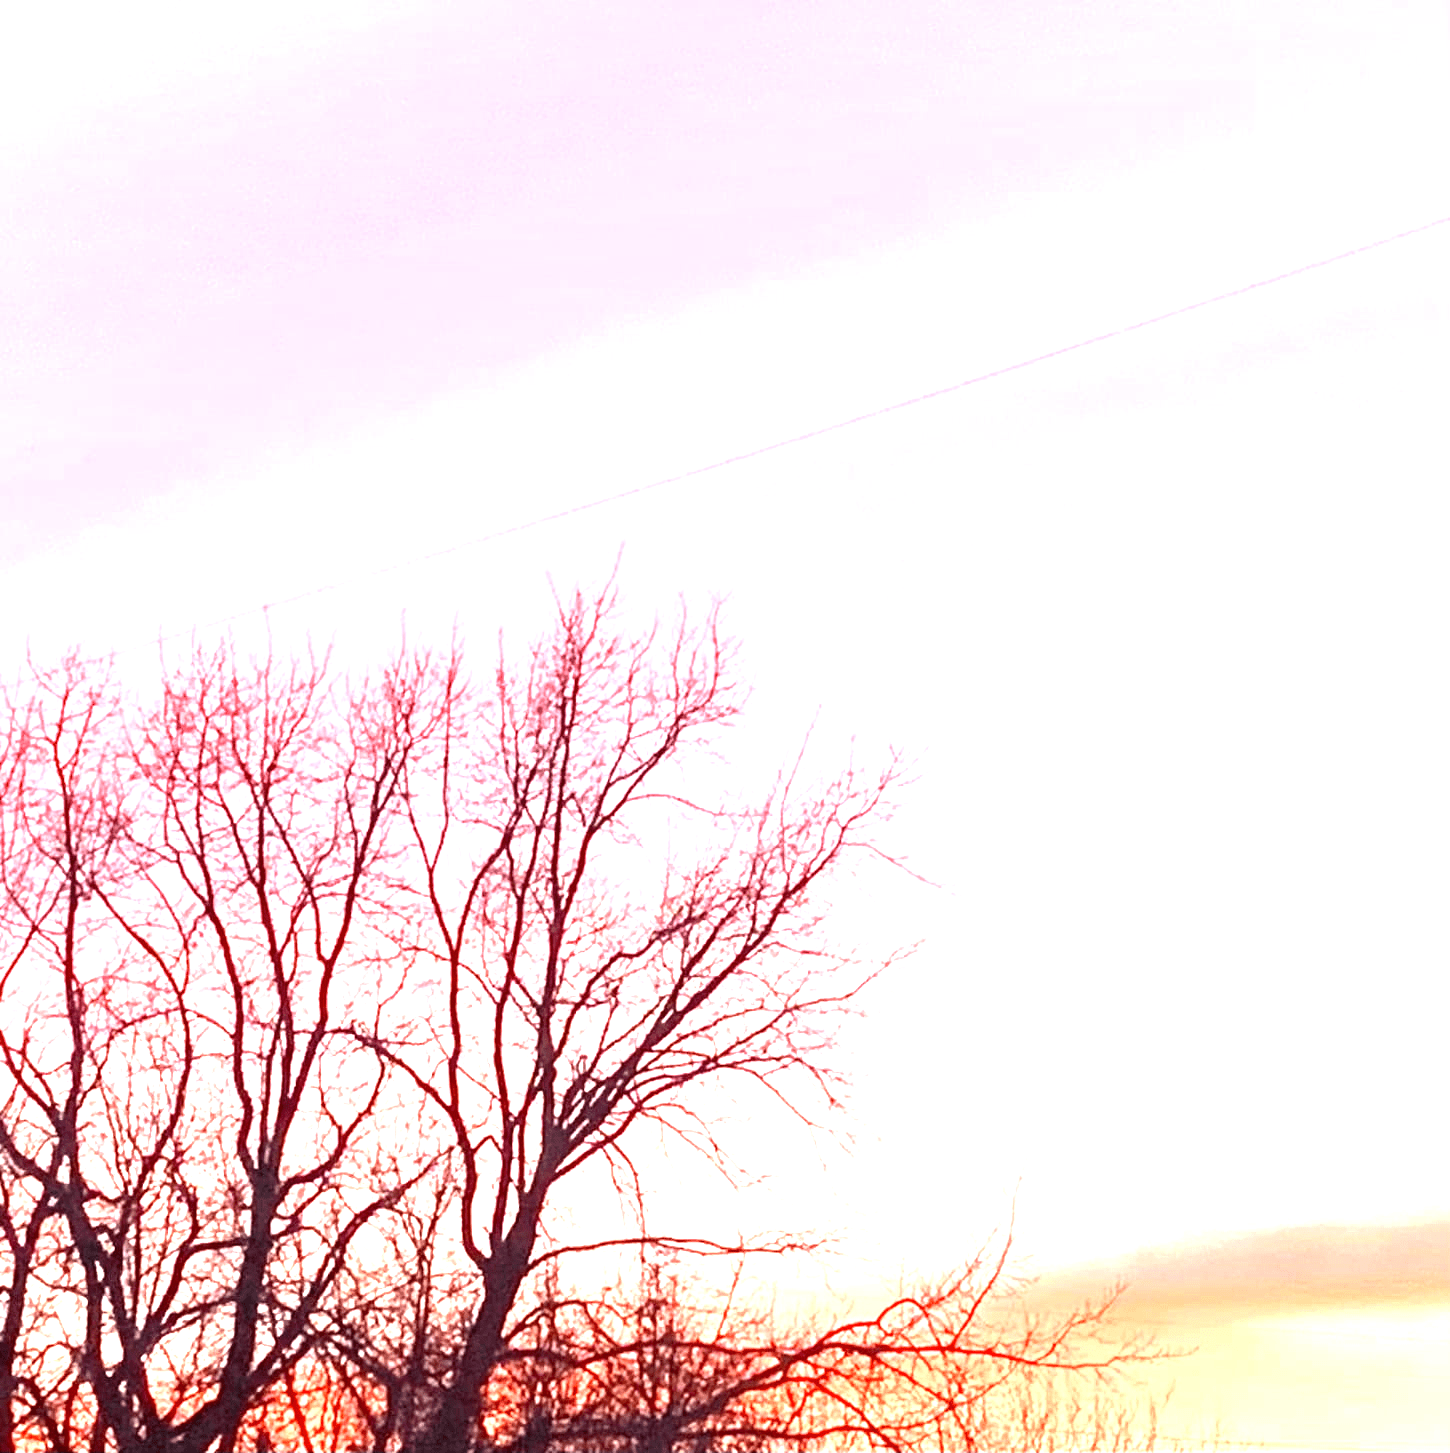
\includegraphics[totalheight = 4cm]{221.png} \hspace{1.5cm}

\includegraphics[totalheight = 4cm]{321.png} \\
{\bf K1 = 2, K2 = 2\/}\\

\includegraphics[totalheight = 4cm]{122.png} \hspace{1.5cm}
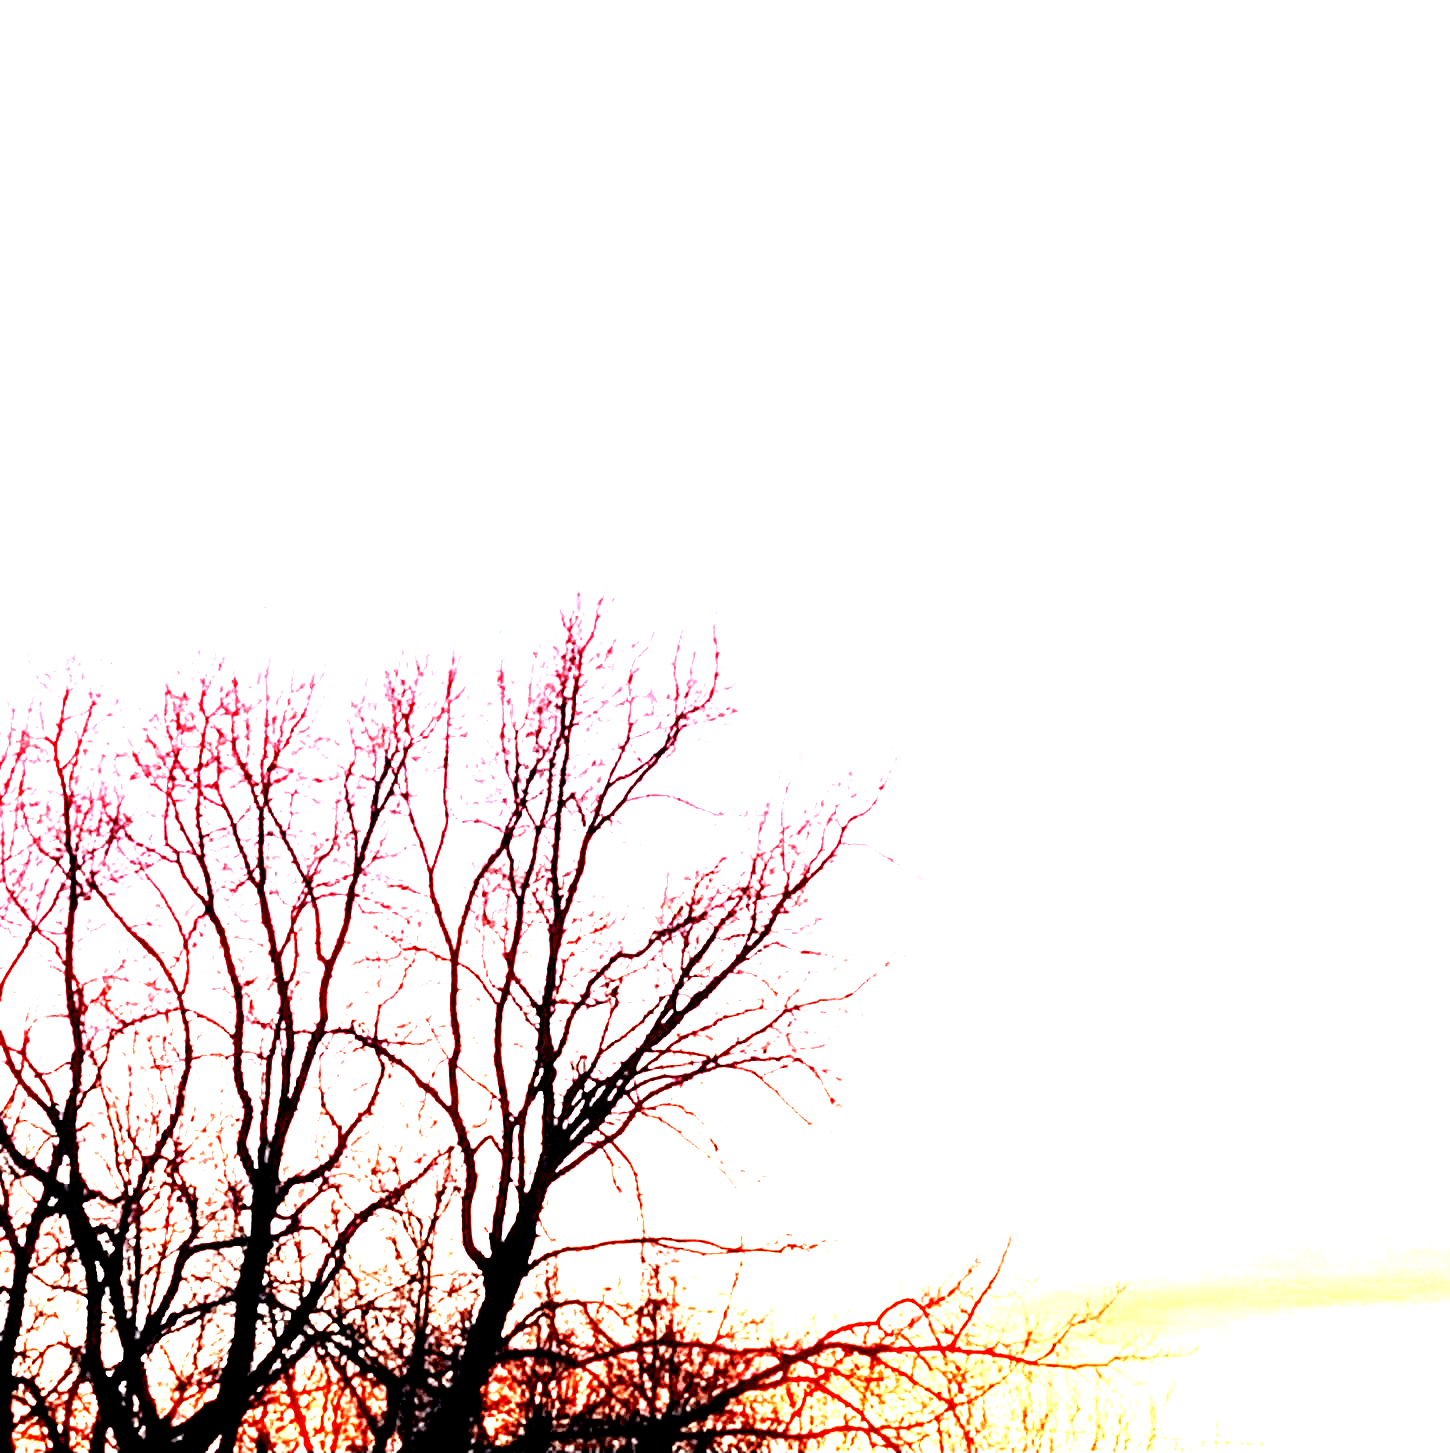
\includegraphics[totalheight = 4cm]{222.png} \hspace{1.5cm}

\includegraphics[totalheight = 4cm]{322.png} \\

\end{document}